\section{Voraussetzungen}

\subsection{Versuchsziel}

In diesem Versuch sollte die Lebensdauer von Myonen vermessen werden. Dafür
wurden verschiedene Logikschaltungen aufgebaut, mit denen die mit
Szintillationszählern registrierten Signale untersucht werden konnten. Aus dem
resultierenden Zeit-Intensitäts-Spektrum kann man dann die Halbwertszeit
ableiten.

\subsection{Physikalische Grundlagen}

Die hier untersuchten Teilchen stammen aus der kosmischen Höhenstrahlung. Aus dem Weltall zur Erde gelangende Protonen wechselwirken mit Atomkernen der
oberen Atmosphäre, woraufhin ein Teilchenschauer entsteht, der hauptsächlich
aus Pionen besteht. Die geladenen $π^{\pm}$ wiederum zerfallen nach
\cite[Gl.16]{script} größtenteils in
$μ^{\pm}$ und die dazugehörigen (Anti-) Neutrinos:
\begin{eqnarray}
π^+ &\rightarrow& μ^+ + ν_μ\\
π^- &\rightarrow& μ^- + \overline{ν}_μ
\end{eqnarray}
Diese Myonen besitzen eine Lebensdauer von ca. \SI{2}{\micro\second} und
üblicherweise eine Geschwindigkeit, die fast der Lichtgeschwindigkeit
entspricht. Nach klassischer Rechnung würden die Myonen im Schnitt also nur
etwa 600m weit kommen, aber durch die relativistische Zeitdilatation, die die
Myonen von der Erde aus gesehen erfahren, gelangen sie trotzdem bis zu uns.

Die Myonen selbst zerfallen wiederum fast ausschließlich wie folgt (s.
\cite[Gl.5]{script}):
\begin{eqnarray}
μ^+ &\rightarrow& e^+ + ν_l + \overline{ν}_μ\\
μ^- &\rightarrow& e^- + \overline{ν}_e + ν_μ
\end{eqnarray}
Dabei liegt die Halbwertszeit $τ_μ$ nach \cite[Gl.4]{script} bei
\begin{equation}
τ_μ = \SI{2,19703(4)}{\micro\second} 
\label{eqn:tau_mu_theo}
\end{equation}
Diese Größe werden wir versuchen zu verifizieren.

\subsection{Versuchsaufbau}

Der Detektoraufbau, der in \fref{detector} dargestellt ist, wurde
\cite[Abb.3]{script} entnommen.
\begin{figure}[htb]
     \centering
     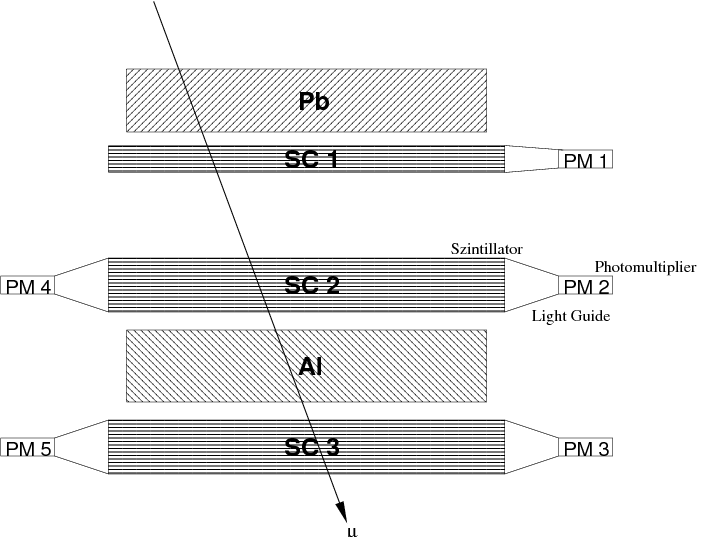
\includegraphics[width=1\columnwidth,keepaspectratio]{../docs/detector.png}
     \caption{Detektoraufbau}
     \label{fig:detector}
\end{figure}
Man kann in diesem Bild erkennen, dass sich oben über dem ersten
Szintillationszähler SC1 ein großer Bleiblock befindet, der dafür sorgt, dass
von oben keine anderen Teilchen außer Myonen den Detektor erreichen. Dies
funktioniert, da alle anderen Teilchen beim Durchgang durch Materie entweder
mehr Energie durch Bremsstrahlung oder durch Ionisationsverluste verlieren als
Myonen es tun. Der Szintillationszähler SC1 registriert also die eintreffenden
Myonen, und da diese annähernd Lichtgeschwindigkeit besitzen, werden sie auch
im Rahmen der Detektor-Zeitauflösung zeitgleich im Szintillationszähler SC2
registriert. Anschließend müssen die Teilchen einen Aluminiumblock passieren,
der sie so stark abbremst, dass man davon ausgehen kann, dass sie zur Ruhe
gekommen sind. In SC3 sollte also zunächst kein Signal beobachtet werden. Die
Myonen, die wir selektieren möchten, zerfallen also zwischen SC2 und SC3. Das
beim Zerfall ausgesendete (Anti-) Elektron muss mit einer Zeitverzögerung in
SC3 detektiert werden (es wäre auch möglich, dass es in SC2 gemessen wird, aber
unsere Logikschaltung selektiert nur den ersten Fall.)

Um die erwähnten (Anti-) Koinzidenzen zu gewährleisten, haben wir Abfolgen von
UND- und ODER-Schaltungen verwendet.

Wie in vielen Experimenten muss man versuchen, den Untergrund zu minimieren.
Eine von uns umgesetzte Methode ist die Forderung einer Koinzidenz in den
beiden zu einem Szintillationszähler gehörenden Photomultipliern (PM 2 und PM 4
für SC2 und PM 3 und PM 5 für SC3). Dies reduziert den Einfluss von zufällig in
den Photomultipliern thermisch ausgelösten Elektronen, da diese kaum
gleichzeitig in beiden PMs auftreten werden.

\subsection{Verwendete Geräte}

Für die Versuchsdurchführung wurde der im \cite{script} vorgeschlagenen und
bereits vorbereitete Aufbau verwendet. Das wären im Einzelnen die folgenden
Geräte:
\begin{itemize}
\item Plastikszintillatoren NE102A
\item Photomultiplier H7360-02
\item Koaxialkabel RG58U
\item Liste der NIM- und Elektronikmodule: s. \cite[Anhang B]{script}
\end{itemize}